\section{论证的分析}

\begin{quotation}
\textit{论证分析是逻辑学中至关重要的技能,通过系统的分析方法可以清晰地展现复杂论证的结构和逻辑关系。}
\end{quotation}

许多论证是简单的,但有些论证却相当复杂。论证的前提可以用各种不同方式支持其结论。论证中前提的数量和命题顺序也有所不同。我们需要关于论证性话语的一些分析技法,借以澄清前提与结论的关联。

通常有两种分析技法用于论证分析。一种是\textbf{解析}(paraphrase),即用清楚的语言和逻辑顺序表明论证中的命题;另一种是\textbf{图示}(diagram),用二维空间关系图展示论证的结构。两种技法都很有用,可根据不同情况选用最方便适用的一种。

\subsection{解析法}

考虑下面这个多于两个前提的论证的原初表述:

\begin{quotation}
现代鸟类并非从直立行走的兽脚类恐龙(包括霸王龙)进化而来,有三个主要理由。首先,大多数类鸟兽脚类恐龙化石发源时间比初始鸟类遗留的化石晚七千五百万年。……其次,鸟的祖先必定已适宜飞行,而兽脚类恐龙并不适宜飞行。第三个理由在于……兽脚类恐龙都有锯状牙齿,而鸟类没有锯状牙齿。${}^{[10]}$
\end{quotation}

我们可通过解析澄清该论证,即利用清楚简明的语言列出其每一个前提及结论:

\begin{enumerate}
  \item 类鸟兽脚类恐龙化石比初始鸟类遗留的化石发源时间要晚得多。
  \item 鸟的祖先必定已适宜飞行,但兽脚类恐龙不适宜飞行。
  \item 兽脚类恐龙都有锯状牙齿,而鸟类没有锯状牙齿。\\
  所以,现代鸟类并非从直立行走的兽脚类恐龙进化而来。
\end{enumerate}

对论证的分析通常能帮助我们更好地理解论证,因为做这样的分析必须把在论证中被假定但没有充分明晰地陈述的东西揭示出来。譬如大数学家哈代曾有如下论说:

\begin{quotation}
阿基米得将被永远记住而埃斯库罗斯会被遗忘,因为一种语言会消亡而数学理念不会消亡。${}^{[11]}$
\end{quotation}

对该论证的充分的分析,需清楚地表明其所承诺的东西:

\begin{enumerate}
  \item 一种语言会消亡。
  \item 埃斯库罗斯的伟大剧作使用一种语言。
  \item 故埃斯库罗斯的成果终究会消亡。
  \item 数学理念不会消亡。
  \item 阿基米得的伟大工作使用数学理念。
  \item 故阿基米得的成果不会消亡。\\
  所以,阿基米得将被永远记住而埃斯库罗斯将被遗忘。
\end{enumerate}

这种分析使我们看到,哈代这一短句之中,浓缩了几个带有可疑前提的论证。

\subsection{图示法}

有时运用图示展示一个论证的结构是非常有益的。其步骤是给论证中出现的每一个命题逐次赋予一个置于圆圈中的数字,然后在数字间使用箭头符号展示其中前提与结论的逻辑关联。这样可避免像解析法那样重述前提。考虑如下论证:

\begin{quotation}
(1)与许多人的认识相反,HIV检测呈阳性并不必定是死亡判决。一方面,(2)从(艾滋病病毒)抗体生发到出现临床症状平均将近十年时间;另一方面,(3)许多研究报告显示,相当数量的检测呈阳性者从未发展为艾滋病患者。${}^{[12]}$
\end{quotation}

不用重述论证中的命题,使用标示命题的圆圈数字即可把该论证图示如下:

\begin{center}
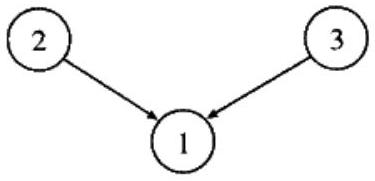
\includegraphics[width=\textwidth]{images/2025_05_15_6a28331d5e7c993ad07ag-030.jpg}
\end{center}

如果一个论证是简单直接的,则完全不需要借助图示去理解它。然而论证往往不是直接的,而图示法能够在平面图上直观地显示论证的结构,因而是非常有用的。${}^{[13]}$ 我们在图中把\textbf{结论}置于\textbf{前提}的下方,而论证的所有前提都在图中的同一行上列出。

与解析法相比,图示法更易于展现论证的前提支持结论的方式。例如在上面这个论证中,前提(2)和(3)都分别独立地支持结论(1):HIV检测呈阳性并不必定是死亡判决。就是说,每个前提自身都为接受结论提供了某种理由,即使没有另一个前提也不影响其为结论所提供的支持。这种\textbf{分立性支持}直观地展现在图示之中。

但是,在有些论证中,只有把前提结合在一起才能达到支持结论的目的。例如:

\begin{quotation}
(1) 我们应该允许安乐死,(2) 如果这样做是最适当地维护所有当事人的利益的话。(3) 而有时候安乐死确实是最适当地维护所有当事人的利益。(4) 因此我们有时候应该允许安乐死。${}^{[14]}$
\end{quotation}

该论证的正确图示将展现出只有当前提之间相结合才能支持结论,即:

\begin{center}
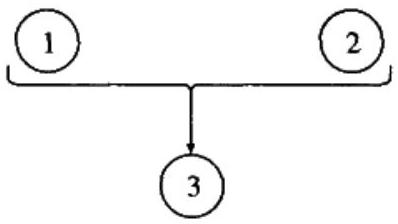
\includegraphics[width=\textwidth]{images/2025_05_15_6a28331d5e7c993ad07ag-031(1).jpg}
\end{center}

此处我们用\textbf{托架线}置于前提之下,是因为在这个例子中两个前提都不能独立地支持结论。如果第一个前提表达的原则是真的,但不存在能够最适当地维护所有当事人的利益的安乐死事例,则结论就根本没有得到支持。而如果的确存在能够最适当地维护所有当事人的利益的安乐死情形,但第一个前提所表述的原则是错误的,则结论仍然没有获得支持。

\subsection{复杂论证的分析}

当论证有更复杂的结构时,图示法就显得特别有用。有时可以很容易地展示出原本很难说清楚的东西。考虑如下论证:

\begin{displayquote}
(1)沙漠高地是天文观测的良好场所。(2)其高度使得它们坐落于大气层之中,使得星光不用穿越整个大气层而到达望远镜。(3)沙漠的干燥度也使之相对较少受云雾干扰。(4)云雾对天空的遮蔽会使许多天文观测归于无用。${}^{[15]}$
\end{displayquote}

命题(1)显然是这个论证的结论,其他三个命题提供对它的支持,但它们支持结论的方式是不一样的。命题(2)自身即可支持沙漠高地是天文观测良好场所的断言,而命题(3)和(4)必须联合起来才能支持这个断言。如下图示可清楚地表明这一点:

\begin{center}
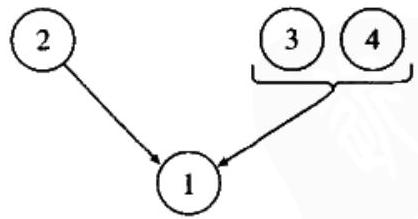
\includegraphics[width=\textwidth]{images/2025_05_15_6a28331d5e7c993ad07ag-031.jpg}
\end{center}

但是某些复杂论证结构的澄清使用解析法更为奏效。例如,当一个论证含有未明确陈述出来的\textbf{隐含前提}时,解析法允许我们直接把隐含前提列出,而图示法则需要既列出隐含前提又要以某种直观形式(如非封闭圆圈)表明它是被附加到原来论说之上的。请考虑如下论证:

\begin{quotation}
只有当我能够做出其他选择时,我对我的行为才负有道德责任。因为一个人若无力避免某行为,就不应被认为对该行为负有道德责任。${}^{[16]}$
\end{quotation}

运用列出隐含前提的解析法,该论证很容易澄清如下:

\begin{enumerate}
  \item 一个人若无力避免某行为,就不应被认为对该行为负有道德责任。
  \item 只有当我能够做出其他选择时,我当下的行为才是我有能力避免的。\\
  所以,只有当我能够做出其他选择时,我对我的行为才负有道德责任。
\end{enumerate}

\subsection{多重复合论证}

当一段话包含两个或更多论证和若干相互关联并不明显的命题时,图示法被证明特别有用。下面是从马克思给恩格斯的一封信中摘录的一段话:

\begin{displayquote}
(1)加速英国的社会革命就是国际工人协会的最重要的目标。(2)而加速这一革命的唯一办法就是使爱尔兰独立。因此,(3)国际的任务就是到处把英国和爱尔兰的冲突提到首要地位,(4)到处都公开站在爱尔兰方面。${}^{[17]}$
\end{displayquote}

一段话中论证的数目通常取决于其中所含结论的数目。这段话中含有两个结论,因而有两个论证。但这两个结论都是从同样的两个前提推得的,如下图示可很好地展示这种结构:

\begin{center}
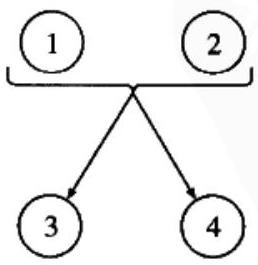
\includegraphics[width=\textwidth]{images/2025_05_15_6a28331d5e7c993ad07ag-032.jpg}
\end{center}

有时,含有两个结论从而有两个论证的一段话,却只含有一个前提。例如:

\begin{quotation}
年纪较大的妇女更难以抵制工作中的性骚扰和离开施暴的丈夫,因为年龄的偏见使她们不容易找到其他保护自己的方式。${}^{[18]}$
\end{quotation}

其中唯一的前提是年纪较大的妇女不容易找到保护自己的方式。该前提支持两个结论:年纪较大的妇女难以抵制工作中的性骚扰,以及她们(对已婚妇女而言)难以离开施暴的丈夫。我们通常用"\textbf{单独论证}"一词指谓只有一个结论的论证,而不管有多少用以支持它的前提。

\subsection{论证中的命题次序}

当一段话中出现两个或更多论证,或一个论证中有两个或更多前提时,就需要弄清各个前提及结论出现的次序。结论可能在最后或最先出现,也可能出现在用以支持它的前提之间,如下例:

\begin{quotation}
穆斯林思想家启示的真正来源是《古兰经》及神圣先知的言论。因而很显然,穆斯林哲学并不是希腊思想的复制品,其所关心的主要是那些来自穆斯林和与穆斯林相关的特定问题。${}^{[19]}$
\end{quotation}

这段话中的结论"穆斯林哲学并不是希腊思想的复制品",出现在论证的第一个前提之后和第二个前提之前。

\subsection{串联式论证}

同一个命题既可在一个论证中做结论,又可在另一个论证中做前提,正如同一个人既可在一个场合做指挥者,又可在另一个场合做被指挥者。托马斯·阿奎那的著作中有一段话可以很好地说明这一点。他说:

\begin{displayquote}
人类的法律是为人类大众制定的,\\
大多数人在德行上是不完美的,\\
因此人类的法律不禁止一切罪恶。${}^{[20]}$
\end{displayquote}

该论证的结论随即被托马斯·阿奎那用做另一个完全不同的论证的前提:

\begin{displayquote}
恶行与善行相反,\\
但人类的法律不禁止一切罪恶,\\
因此人类的法律也不规定一切善行。${}^{[21]}$
\end{displayquote}

\subsection{浓缩论证的分析}

当一系列复杂的论证关系被压缩,对于这样一串浓缩论证的分析,完全解析法会提供很大的帮助。考虑如下论证集合:

\begin{quotation}
因为(1)出现在非洲人种身上的线粒体变种最多,科学家推断,(2)非洲人种的进化史最长,这表明(3)非洲人种可能是现代人类的起源。${}^{[22]}$
\end{quotation}

我们可以把这段论证图示如下:

\begin{center}
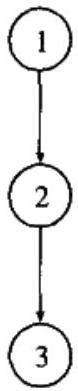
\includegraphics[width=\textwidth]{images/2025_05_15_6a28331d5e7c993ad07ag-034.jpg}
\end{center}

而对这同一串论证的分析,解析法尽管显得不够简洁,但更完整:

\begin{enumerate}
  \item 一个人种身上的线粒体变种越多,其进化史就越长;
  \item 出现在非洲人种身上的线粒体变种最多,\\
  因此非洲人种进化史最长。
\end{enumerate}

\begin{enumerate}
  \item 非洲人种进化史最长,
  \item 现代人类可能起源于进化史最长的人种,\\
  因此现代人类可能起源于非洲人种。
\end{enumerate}

这样的复合论证表明,一个孤立表达的命题既非前提也非结论。在一个论证中,作为假定出现的命题就是前提,被断定为从假定命题推出的命题就是结论。也就是说,"\textbf{前提}"和"\textbf{结论}"都是相对的(relative)术语。

\subsection{交织式论证}

几个论证复合在一起,语言表达上可能不是以串联的方式出现,而是以独特的方式相互交织,这就要求我们对它们做细致的分析。图示法特别适用于这种情况。例如,在约翰·洛克的名篇《政府论》中,下面一段话就有两个论证交织在一起:

\begin{quotation}
立法机构常年运作是不必要的,也是很不方便的;但行政机关常年运作是绝对必要的,因为不是总需要制定新的法律,但总需要执行已制定的法律。
\end{quotation}

上述论证的分支命题可以用数字表示为:(1)立法机构常年运作是不必要的,也是很不方便的,(2)行政机关常年运作是绝对必要的,(3)不是总需要制定新的法律,(4)总需要执行已制定的法律。将这段论证图示如下:

\begin{center}
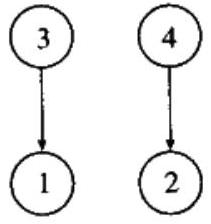
\includegraphics[width=\textwidth]{images/2025_05_15_6a28331d5e7c993ad07ag-035.jpg}
\end{center}

这个图示表明,第二个论证的结论出现在第一个论证的结论和前提之间,第一个论证的前提出现在第二个论证的结论和前提之间。这个图示还表明,两个结论都出现在它们的前提之前。

这个图示同样也展示了支持刑罚威慑理论的古罗马哲学家塞涅卡的两个相关论证的逻辑结构:
\begin{quotation}
(1)惩罚罪行不是因为罪行已经发生,(2)而是为了不发生新的罪行。[因为](3)过去的罪行不能被取消,(4)但是可以预防将来的罪行。
\end{quotation}

在这段话中,"惩罚罪行不是因为罪行已经发生"是其中一个论证的结论,其前提是"过去的罪行不能被取消"。"惩罚罪行是为了不发生新的罪行"是这段话中第二个论证的结论,其前提是"惩罚罪行可以预防将来的罪行"。

\begin{center}
\fbox{\parbox{0.9\textwidth}{
  \centering
  \textbf{论证分析的工具}\\
  解析法和图示法是两种有力的分析工具,运用这两种工具对论证进行分析,\\
  可以更彻底地理解论证前提与结论的关联。
}}
\end{center} 